\documentclass{beamer}
\mode<presentation> {
\usepackage{color}
\definecolor{bottomcolour}{rgb}{0.21,0.11,0.21}
\definecolor{middlecolour}{rgb}{0.21,0.11,0.21}
\setbeamercolor{structure}{fg=white}
\setbeamertemplate{frametitle}[default]%[center]
\setbeamercolor{normal text}{bg=black, fg=white}
\setbeamertemplate{background canvas}[vertical shading]
[bottom=bottomcolour, middle=middlecolour, top=black]
\setbeamertemplate{items}[circle]
\setbeamertemplate{navigation symbols}{} %no nav symbols
\setbeamercolor{block title}{use=structure,fg=white,bg=structure.fg!50!red!50!blue!100!green}
\setbeamercolor{block body}{parent=normal text,use=block title,bg=block title.bg!5!white!10!bg,fg=white}
\setbeamertemplate{navigation symbols}{}
}
\usepackage{graphicx} 
\usepackage{booktabs} 
\usepackage[utf8]{inputenc}  
\usepackage[T1]{fontenc}  
\usepackage{geometry}     
%\usepackage[francais]{babel} 
\usepackage{eurosym}
\usepackage{verbatim}
\usepackage{ragged2e}
\justifying

%%%%%%%%%%%%%%%%%%%%%%%%%%%%%%%%%%%%%%%%%%%%%%%%%%%%%%%%%%%%%%%%
%% ccBeamer 0.1, 2007-07-02                                   %%
%% Written by Sebastian Pipping <webmaster@hartwork.org>      %%
%% ---------------------------------------------------------- %%
%% Licensed under Creative Commons Attribution-ShareAlike 3.0 %%
%% http://creativecommons.org/licenses/by-sa/3.0/             %%
%%%%%%%%%%%%%%%%%%%%%%%%%%%%%%%%%%%%%%%%%%%%%%%%%%%%%%%%%%%%%%%%


%% Images
\newcommand{\CcImageBy}[1]{%
	
\includegraphics[scale=#1]{creative_commons/cc_by_30.pdf}%
}
\newcommand{\CcImageCc}[1]{%
	
\includegraphics[scale=#1]{creative_commons/cc_cc_30.pdf}%
}
\newcommand{\CcImageDevNations}[1]{%
	
\includegraphics[scale=#1]{creative_commons/cc_dev_nations_30.pdf}%
}
\newcommand{\CcImageNc}[1]{%
	
\includegraphics[scale=#1]{creative_commons/cc_nc_30.pdf}%
}
\newcommand{\CcImageNd}[1]{%
	
\includegraphics[scale=#1]{creative_commons/cc_nd_30.pdf}%
}
\newcommand{\CcImagePd}[1]{%
	
\includegraphics[scale=#1]{creative_commons/cc_pd_30.pdf}%
}
\newcommand{\CcImageSa}[1]{%
	
\includegraphics[scale=#1]{creative_commons/cc_sa_30.pdf}%
}
\newcommand{\CcImageSampling}[1]{%
	
\includegraphics[scale=#1]{creative_commons/cc_sampling_30.pdf}%
}
\newcommand{\CcImageSamplingPlus}[1]{%
	
\includegraphics[scale=#1]{creative_commons/cc_sampling_plus_30.pdf}%
}


%% Groups
\newcommand{\CcGroupBy}[1]{% zoom
	\CcImageBy{#1}%
}
\newcommand{\CcGroupByNc}[2]{% zoom, gap
	\CcImageBy{#1}\hspace*{#2}\CcImageNc{#1}%
}
\newcommand{\CcGroupByNcNd}[2]{% zoom, gap
	\CcImageBy{#1}\hspace*{#2}\CcImageNc{#1}\hspace*{#2}\CcImageNd{#1}%
}
\newcommand{\CcGroupByNcSa}[2]{% zoom, gap
	\CcImageBy{#1}\hspace*{#2}\CcImageNc{#1}\hspace*{#2}\CcImageSa{#1}%
}
\newcommand{\CcGroupByNd}[2]{% zoom, gap
	\CcImageBy{#1}\hspace*{#2}\CcImageNd{#1}%
}
\newcommand{\CcGroupBySa}[2]{% zoom, gap
	\CcImageBy{#1}\hspace*{#2}\CcImageSa{#1}%
}
\newcommand{\CcGroupDevNations}[1]{% zoom
	\CcImageDevNations{#1}%
}
\newcommand{\CcGroupNcSampling}[2]{% zoom, gap
	\CcImageNc{#1}\hspace*{#2}\CcImageSampling{#1}%
}
\newcommand{\CcGroupPd}[1]{% zoom
	\CcImagePd{#1}%
}
\newcommand{\CcGroupSampling}[1]{% zoom
	\CcImageSampling{#1}%
}
\newcommand{\CcGroupSamplingPlus}[1]{% zoom
	\CcImageSamplingPlus{#1}%
}


%% Text
\newcommand{\CcLongnameBy}{Attribution}
\newcommand{\CcLongnameByNc}{Attribution-NonCommercial}
\newcommand{\CcLongnameByNcNd}{Attribution-NoDerivs}
\newcommand{\CcLongnameByNcSa}{Attribution-NonCommercial-ShareAlike}
\newcommand{\CcLongnameByNd}{Attribution-NoDerivs}
\newcommand{\CcLongnameBySa}{Attribution-ShareAlike}

\newcommand{\CcNote}[1]{% longname
	This work is licensed under the \textit{Creative Commons #1 3.0 License}.%
}


\title[Reprenons le contrôle de notre vie privée sur Internet]{Reprenons le contrôle de notre vie privée \\sur Internet} 
\author{Genma}

\begin{document}

%% Titlepage
\begin{frame}
	\titlepage
	\vfill
	\begin{center}
		\CcGroupByNcSa{0.83}{0.95ex}\\[2.5ex]
		{\tiny\CcNote{\CcLongnameByNcSa}}
		\vspace*{-2.5ex}
	\end{center}
\end{frame}

\begin{frame}
\frametitle{
\includegraphics[scale=0.4]{./images/Genma.jpg} \ \ \  A propos de moi  }
\begin{columns}[c] 
\column{.55\textwidth} 
\textbf{Où me trouver sur Internet?}
\begin{itemize}
\item Le Blog de Genma : http://genma.free.fr
\item Twitter : http://twitter.com/genma
\end{itemize}
\textbf{Mes projets-contributions}
\\ Plein de choses dont :
\begin{itemize}
\item Des conférences sur plein de thèmes différents
%\item A.I.\up{2} Apprenons l'Informatique, Apprenons Internet
\end{itemize}
\column{.5\textwidth} 
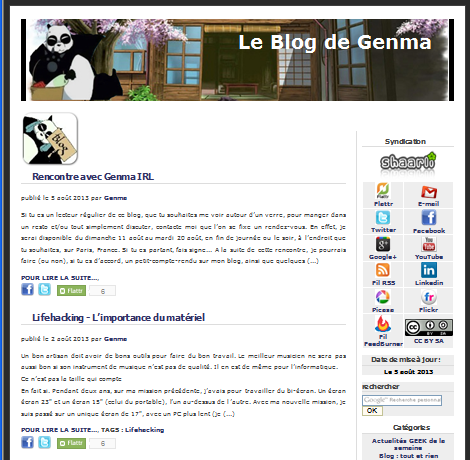
\includegraphics[width=5cm,height=5cm]{./images/blog.png} 
\end{columns}
\end{frame}

%----------------------------------------------------------------------------------------
\begin{frame}
\begin{center}
\Huge{Internet, c'est quoi ?}
\end{center}
\end{frame}

%----------------------------------------------------------------------------------------
\begin{frame}
\frametitle{Internet, un réseau de réseau}
\begin{itemize}
\justifying{
\item Internet c'est un réseau de réseaux d'ordinateurs connectés entre eux.
\item Il y a d'un côté les serveurs, des gros ordinateurs, sur lesquels il y a des sites Internet.
\item Et de l'autre, il y a "nous", avec notre PC, notre tablette, notre smartphone...
}
\end{itemize}
\end{frame}

\begin{frame}
\Huge{\centerline{Toutes ces traces qu'on laisse}}
\Huge{\centerline{sur Internet... sans le savoir}}
\end{frame}

%----------------------------------------------------------------------------------------
\begin{frame}
\begin{center}
\Huge{Toutes ces informations \\ que l'on donne... }
\Huge{Volontairement...}
\Huge{ou pas}
\end{center}
\end{frame}

%----------------------------------------------------------------------------------------
\begin{frame}
\frametitle{Les traces de navigation \emph{locales}}

\begin{block}{Quand on va sur \emph{Internet}}
\justifying{
Plein de fichiers sont créés : 
\begin{itemize}
\item Historique des pages visitées, 
\item Données saisies dans les formulaires et barres de recherche,
\item Les mots de passe conservés, 
\item La liste des téléchargements, 
\item Les cookies, 
\item Les fichiers temporaires...)
\end{itemize}
}
\end{block}
\justifying{Tout ce que l'on fait depuis son navigateur, est, par défaut, conservé sur notre ordinateur, tablette, smartphone...}
\end{frame}


%----------------------------------------------------------------------------------------
\begin{frame}
\frametitle{Les logs de connexions}

\begin{block}{Les traces laissées sur les sites Internets}
\justifying{
Les serveurs Internet gardent différentes traces dont : 
\begin{itemize}
\item l'adresse IP
\item les heures et dates de connexion
\item les informations saisies...
\item le navigateur, son modèle, le système d'exploitation...
\end{itemize}
}
\end{block}
\end{frame}
%----------------------------------------------------------------------------------------
\begin{frame}
\frametitle{Les traces écrites}

\begin{block}{Sur les réseaux sociaux, les blogs, les forums...}
\justifying{
Sur tous ces comptes que l'on a en ligne : 
\begin{itemize}
\item On commente, on réagit ;
\item On "like" ;
\item On ajoute des photos, des vidéos.
\end{itemize}
}
\end{block}
\justifying{Ce sont autant de traces que l'on peut lier à nous.}
\end{frame}

%----------------------------------------------------------------------------------------
\begin{frame}
\frametitle{L'image que je donne de moi}

\justifying{
\begin{block}{\emph{Googler} "son nom"}
\begin{itemize}
\item Les résultats apparaissant sont-ils bien ceux que l'on souhaite?
\end{itemize}
\end{block}
}
\begin{center}
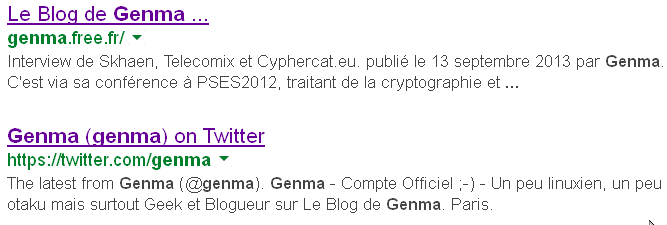
\includegraphics[scale=0.3] {./images/Google01.png}
\\
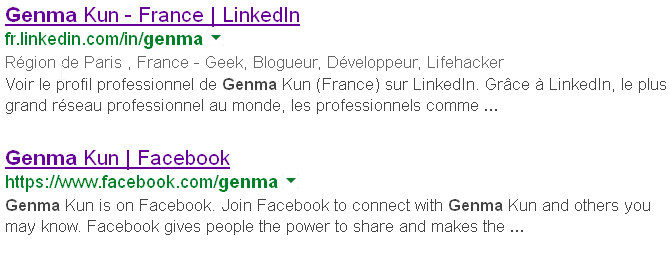
\includegraphics[scale=0.3] {./images/Google02.png}
\end{center}
\end{frame}

%----------------------------------------------------------------------------------------
\begin{frame}
\frametitle{Adage}
\begin{block}{Les paroles s'envolent, les écrits restent}
\begin{itemize}
\justifying{
\item Cet adage est encore plus vrai avec Internet.
\item Il faut partir du principe que ce que l'on dit sera toujours accessible, même des années après.
\item Tout ce qui est sur Internet est public ou le sera (même si c'est "privé". Les conditions d'utilisation évoluent. cf. Facebook).
}
\end{itemize}
\justifying{Rq : Il ne faut donc pas abuser de la liberté d'expression et rester respectueux des lois en vigueur.}
\end{block}
\end{frame}

%----------------------------------------------------------------------------------------
\begin{frame}
\frametitle{Les réseaux sociaux}
\begin{block}{Les données que l'on donne}
\begin{itemize}
\item En remplissant sa fiche Facebook
\item En commentant, en cliquant sur J'aime...
\end{itemize}
\end{block}

\begin{block}{Les données qui sont prises à notre insu}
\begin{itemize}
\justifying{
\item Chaque bouton de partage sur les réseaux sociaux (J'aime etc.) informe le site associé que l'on a consulté tel ou tel site.
\item Les sites associés ont donc une copie de notre historique de consultation de sites Internets (et ce même en mode Navigation privée).
}
\end{itemize}
\end{block}
\end{frame}


\begin{frame}
\frametitle{Illustrations}
\justifying{Des photos de nous en soirée peuvent être mise sur les réseaux sociaux}
\begin{center}

\includegraphics[scale=0.4]{./images/Leak01.jpg}
\end{center}
\end{frame}

\begin{frame}
\frametitle{Illustrations}
\justifying{Parfois aves son smarpthone, on prend des photos plus personnelles...}
\begin{center}

\includegraphics[scale=0.5]{./images/Leak02.png}
\end{center}
\end{frame}

\begin{frame}
\frametitle{Illustrations}
\justifying{Voire des photos \textbf{BEAUCOUP} plus personnelles...}
\begin{center}

\includegraphics[scale=0.5]{./images/Leak03.png}
\end{center}
\end{frame}


%----------------------------------------------------------------------------------------
\begin{frame}
\frametitle{Les mails - courriers électroniques}

\begin{block}{Un mail que l'on envoie, c'est une carte postale}
\justifying{ "On" sait
\begin{itemize}
\item qui écrit à qui ;
\item quand ;
\item pour se dire quoi.
\end{itemize}
}
\justifying{Ex : Gmail lit le contenu des mails pour afficher de la publicité ciblée.}
\end{block}

\begin{block}{Le facteur peut lire la carte postale}
\justifying{ "On" peut
\begin{itemize}
\item envoyer un mail au nom de quelqu'un d'autre ;
\item lire les mails qui circulent sur un réseau...
\end{itemize}
}
\end{block}

\end{frame}
%----------------------------------------------------------------------------------------
\begin{frame}
\frametitle{Les données qui transitent \emph{en clair} sur le Web}
\begin{block}{Quand on consulte un site Internet}
\justifying{
 Le site Internet sait :
\begin{itemize}
\item D'où l'on vient (pays, adresse exacte)
\item La langue que l'on parle, l'heure de l'ordinateur, son modèle...
\end{itemize}
}
\end{block}
\begin{block}{Les connexion http}
\justifying{
Sans le "cadenas" dans la barre d'adresse :
\begin{itemize}
\item Le mot de passe circule "en clair"
\item Avec \emph{un logiciel}, \emph{un pirate} peut récupérer le mot de passe.
\end{itemize}
}
\end{block}
\end{frame}
%----------------------------------------------------------------------------------------
\begin{frame}
\frametitle{Cloud - l'informatique dans les nuages}
\begin{block}{Définition du cloud}
\justifying{
\begin{itemize}
\item Le \emph{Cloud} , c'est l'ordinateur d'un autre.
\end{itemize}
}
\begin{center}

\includegraphics[scale=0.25] {./images/cloud.png} 
\end{center}
\end{block}

\begin{block}{Les \emph{problèmes} du cloud}
\justifying{
Le stockage est gratuit
\begin{itemize}
\item les documents sont analysés (pour de la publicité, de l'espionnage industriel... etc.).
\item Nos données peuvent être piratées et diffusées dans la nature ?
\item Si le service ferme, que deviennent nos données ?
\end{itemize}
}
\end{block}

\end{frame}
%----------------------------------------------------------------------------------------
\begin{frame}
\begin{center}
\Huge{Les métadonnées}\\~\\
\LARGE{Ces données cachées des documents}
\end{center}
\end{frame}

\iffalse%----------------
\begin{frame}
\frametitle{Les métadonnées}
\begin{block}{Qu'est-ce qu'une métadonnée ?}
\justifying{
Une métadonnée est une information qui caractérise une donnée. 
\\~\\
Prenons un exemple : lorsque vous créez un PDF, en général, des données additionnelles sont ajoutées à votre fichier : le nom du logiciel producteur, votre nom, la date de production, la description de votre document, le titre de votre document, la dernière date de modification… ce sont des métadonnées. 
\\~\\
Vous n'avez peut-être pas envie de partager ces informations lorsque vous partagez votre fichier.}
\end{block}
\end{frame}
\fi%----------------
%------------------------------------------------
\begin{frame}
\frametitle{Metadata Photo}
\begin{center}
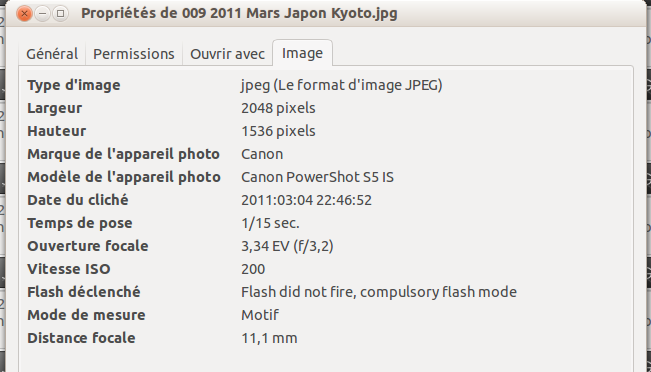
\includegraphics[scale=0.5] {./images/Metadata.png} 
\end{center}
\end{frame}

\begin{frame}
\frametitle{Metadata Photo}
\begin{center}
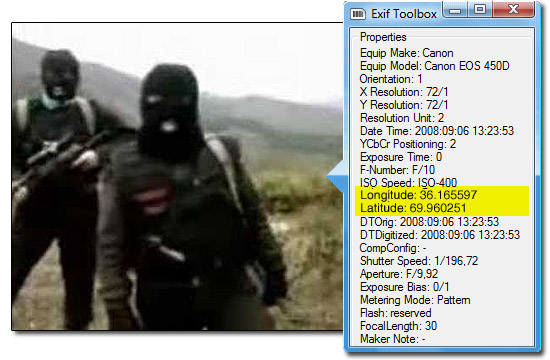
\includegraphics[scale=0.5] {./images/exif-metadata.jpg} 
\end{center}
\end{frame}

\begin{frame}
\frametitle{Géolocalisation des chats}
\begin{center}
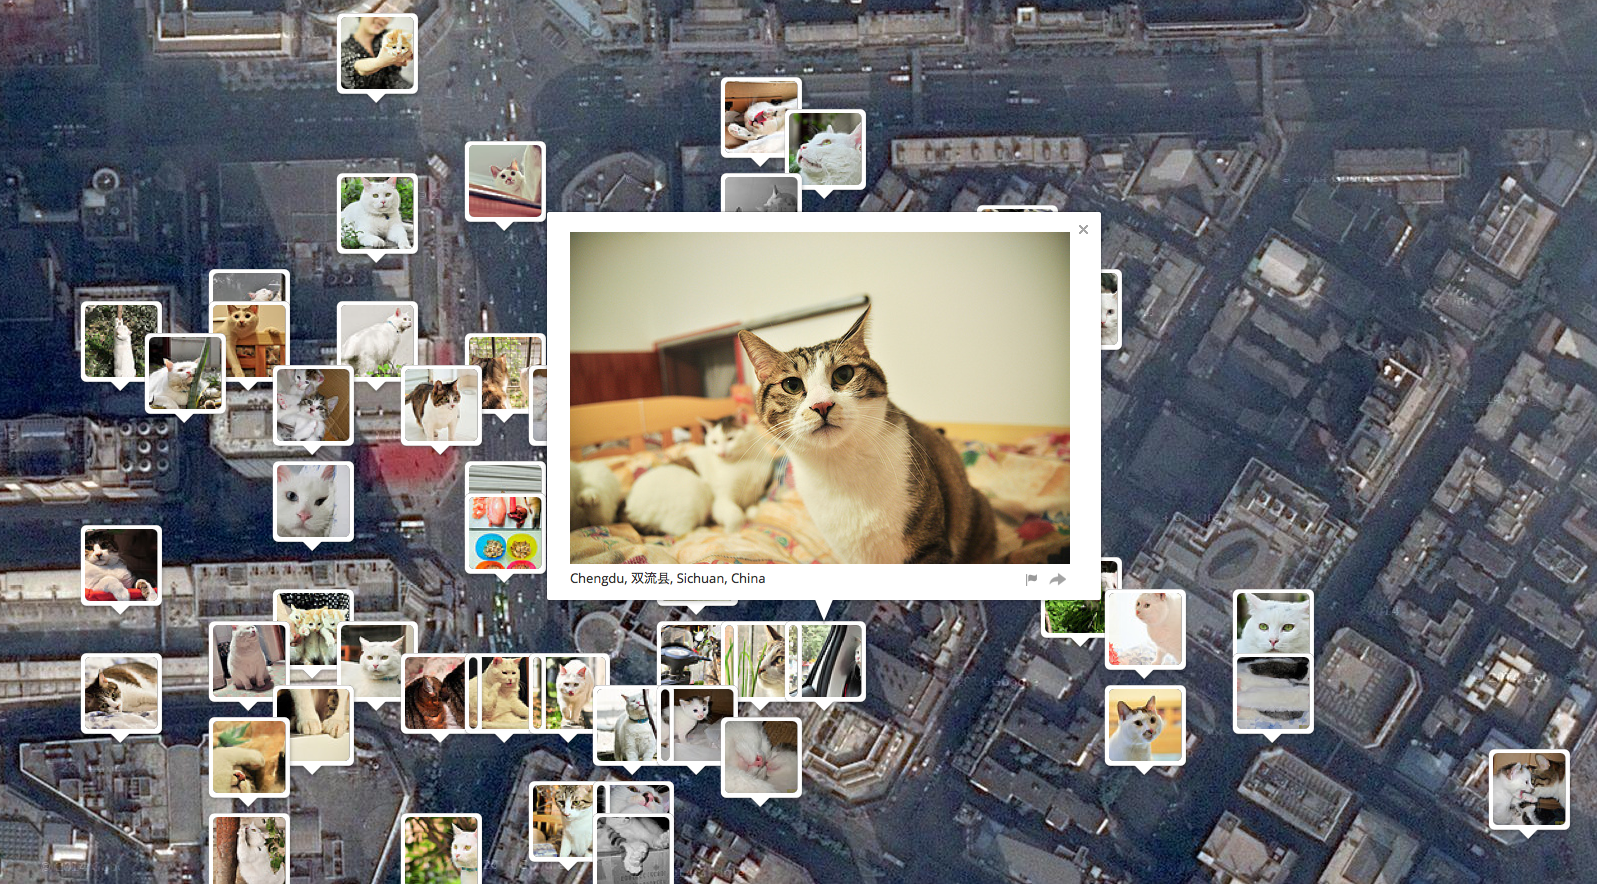
\includegraphics[scale=0.3] {./images/Chat_geolocalisaion.png}
\end{center}
\end{frame}

\begin{frame}
\frametitle{Metadata Word 1/2}
\begin{center}
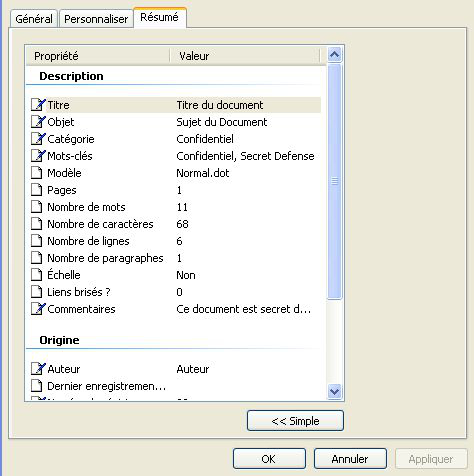
\includegraphics[scale=0.5] {./images/Word01.jpg} 
\end{center}
\end{frame}

\begin{frame}
\frametitle{Metadata Word 2/2}
\begin{center}
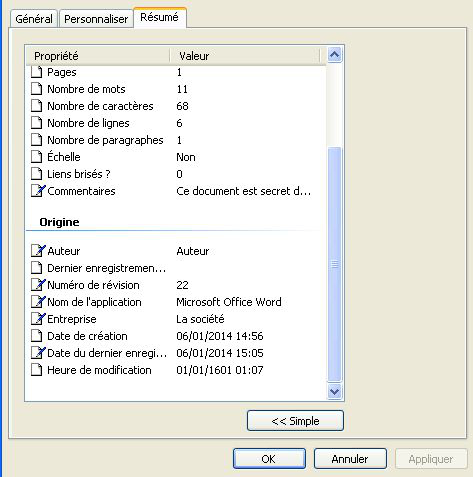
\includegraphics[scale=0.5] {./images/Word02.jpg}
\end{center}
\end{frame}

%------------------------------------------------
\iffalse%----------------
\begin{frame}
\frametitle{Les métadonnées}
\begin{block}{Pourquoi les métadonnées sont-elles un risque pour notre vie privée ?}
\justifying{
Les métadonnées dans un fichier peuvent en dire beaucoup sur vous. Les appareils photos enregistrent des données sur le moment où une photo a été prise et quel appareil photo a été utilisé. 
\\~\\
Les documents bureautiques ajoutent automatiquement l'auteur et diverses informations sur la société aux documents et feuilles de calcul. 
\\~\\
Peut-être que vous ne voulez pas divulguer ces informations sur le Web ?
}
\end{block}
\end{frame}
\fi%----------------

\begin{frame}
\begin{center}
\Huge{Quand on fait une recherche dans Google...}
\end{center}
\end{frame}

%----------------------------------------------------------------------------------------
\begin{frame}
\frametitle{Google}

\begin{block}{Découvrez comment Google vous voit}
\justifying{
Google tente de créer un profil de base de vous, selon votre âge, votre sexe, vos centres d’intérêt. C’est avec ces données que Google vous « sert » des annonces pertinentes. Vous pouvez examiner la façon dont Google vous voit ici  :
\url{https://www.google.com/ads/preferences/}
}
\end{block}

\begin{block}{Découvrez l’historique de votre géolocalisation}
\justifying{
Si vous utilisez Android, votre appareil mobile peut envoyer à Google des informations de géolocalisation et de vitesse de déplacement d’un point à l’autre. Vous pouvez voir l’historique complet de vos « positions » et les exporter ici  :\\
\url{https://maps.google.com/locationhistory}
}
\end{block}
\end{frame}
\begin{frame}
\frametitle{Google}
\begin{block}{Découvrez l’intégralité de votre historique de recherches Google}
\justifying{
Google enregistre jusqu’à la moindre recherche que vous faites. Par-dessus le marché, 
Google enregistre toutes les pubs Google sur lesquelles vous avez cliqué. L’historique est à votre disposition ici  :\\
\url{https://history.google.com}
}
\end{block}
\begin{block}{Découvrez tous les appareils qui ont accédé à votre compte Google}
\justifying{
Si vous craignez que quelqu’un d’autre ait pu utiliser votre compte, vous pouvez trouver la liste de tous les appareils qui ont accédé à votre compte Google, leur adresse IP et leur emplacement approximatif  :\\
\url{https://security.google.com/settings/security/activity}
 }
\end{block}
\end{frame}
\begin{frame}
\frametitle{Google}
\begin{block}{Découvrez toutes les applications et les extensions qui ont accès à vos données Google}
\justifying{
Ceci est une liste de toutes les applications qui ont tout type d’accès à vos données. Vous pouvez voir le type exact de permissions accordées à l’application et révoquer l’accès à vos données en suivant ce lien  :\\
\url{https://security.google.com/settings/security/permissions}
}
\end{block}
\end{frame}

%------------------------------------------------
\begin{frame}
\frametitle{Rien qu'avec les services Google}
\begin{itemize}
\justifying{
\item Google Search
\item GMail 
\item Google Analytics 
\item Google Maps 
\item Smartphone Android 
\item Google Calendar 
\item Google Wallet 
\item Google Docs et Drive 
\item Google Chrome, navigateur 
\item Google Photos 
\item Youtube 
\item ...
}
\end{itemize}
\end{frame}

%----------------------------------------------------------------------------------------
\begin{frame}
\frametitle{Les GAFAM}
GAFAM : Google, Apple, Facebook, Amazon, Microsoft
\begin{itemize}
\justifying{
\item Concentration des acteurs d’Internet autour de silos;
\item Une centralisation nuisible (frein à l'innovation);
\item Les utilisateurs de ces services ne contrôlent plus leur vie numérique.
}
\end{itemize}
\end{frame}


%----------------------------------------------------------------------------------------
\begin{frame}
\begin{center}
\Huge{Sur Internet, si c'est gratuit, c'est VOUS le produit }
\end{center}
\end{frame}
%----------------------------------------------------------------------------------------

\begin{frame}
\frametitle{Comment est-on pisté ?}

\justifying{
\begin{block}{Toutes les publicités nous espionnent}
\begin{itemize}
\item Le bouton Like de Facebook : il permet à FaceBook de savoir que vous avez visité ce site, même si vous n'avez pas cliqué sur ce bouton.
\item Même si vous vous êtes correctement déconnecté de Facebook.
\item De même pour le bouton le +1 de Google, les scripts de Google Analytics, 
\item Tous les publicité, Amazon...
\end{itemize}
\end{block}
}
\begin{center}

\includegraphics[scale=0.3] {./images/Facebook_like.png}
\end{center}
\end{frame}

%----------------------------------------------------------------------------------------
\begin{frame}
\frametitle{Le tracking publicitaire}
\begin{block}{Le pistage sur Internet}
\begin{itemize}
\justifying{
\item Le pistage est un terme qui comprend des méthodes aussi nombreuses et variées que les sites web, les annonceurs et d'autres utilisent pour connaître vos habitudes de navigation sur le Web. 
\item Cela comprend des informations sur les sites que vous visitez, les choses que vous aimez, n'aimez pas et achetez. 
\item Ils utilisent souvent ces données pour afficher des pubs, des produits ou services spécialement ciblés pour vous. 
}
\end{itemize}
\end{block}
\end{frame}

\begin{frame}
\frametitle{Lightbeam}
\begin{center}
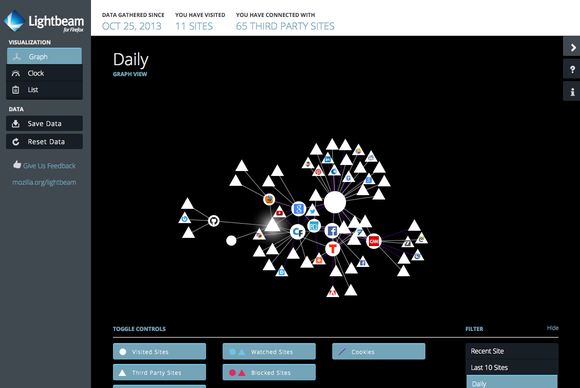
\includegraphics[scale=0.5] {./images/lightbeam.png}
\end{center}
\end{frame}


\begin{frame}
\frametitle{Exemple de la carte de fidélité...}
\justifying{
En magasin, je peux faire le choix de donner ou non ma carte de fidélité et d'être tracé pour un achat.
Sur Internet, par défaut, je suis tracé...
}
\end{frame}

%========================================================================================
\begin{frame}
\Huge{\centerline{Moi, je n'ai rien à cacher}}
\end{frame}

%----------------------------------------------------------------------------------------
\begin{frame}
\frametitle{Différents \emph{modèles de menace}}
\begin{block}{Répondre aux questions}
\justifying{
\begin{itemize}
\item Quelles sont les données et informations que j'estime personnelles - confidentielles? 
\item Qu'est ce que je suis prêt-e à apprendre et à faire pour les protéger?
\end{itemize}
}
\end{block}
Pour se faire un avis \url{http://jenairienacacher.fr/}
\end{frame}

%----------------------------------------------------------------------------------------
\begin{frame}
\Huge{\centerline{Quelques exemples}}
\end{frame}

%------------------------------------------------
\begin{frame}
\frametitle{Le sexe par exemple. C’est perso ou pas ?}

\begin{block}{Billet Tout à cacher par Kiteoa \url{http://reflets.info/}}
\begin{itemize}
\justifying{
\item En 2012, les identifiants et les mots de passe d’utilisateurs de Youporn ont été diffusés sur Pastebin...
}
\end{itemize}
\end{block}
\begin{center}
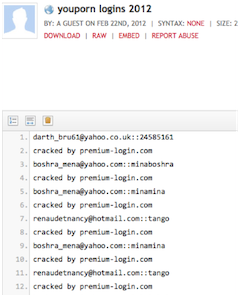
\includegraphics[scale=1]{./images/youporn.png}
\end{center}
\end{frame}

%------------------------------------------------
\begin{frame}
\frametitle{Le sexe par exemple. C’est perso ou pas ?}

\begin{block}{Billet Tout à cacher par Kiteoa \url{http://reflets.info/}}
\begin{itemize}
\justifying{
\item Une boutique en ligne de type sexshop s'est fait piratée... Chacun a le droit de garder pour lui le fait qu’il achète (ou pas) des surtout si « chacun » a utilisé son mail professionnel pour passer commande…}
\end{itemize}
\end{block}
\begin{center}
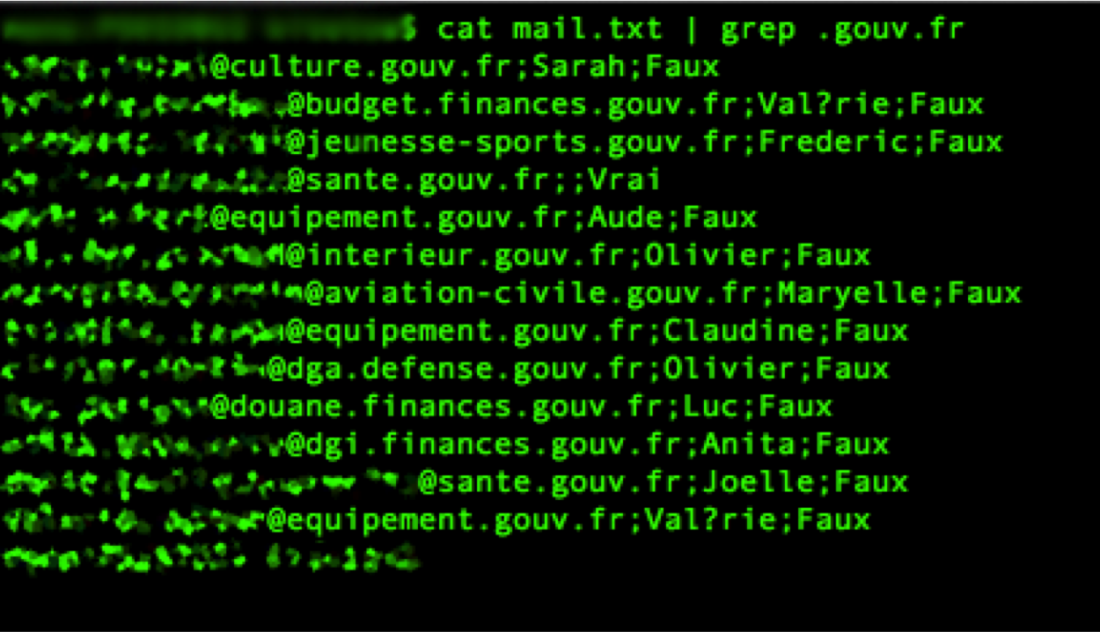
\includegraphics[scale=1]{./images/lesexshopquivamal.png}
\end{center}
\end{frame}

%----------------------------------------------------------------------------------------
\begin{frame}
\Huge{\centerline{L'espionnage}}
\end{frame}

\begin{frame}
\frametitle{L'espionnage 1/2}
\begin{center}
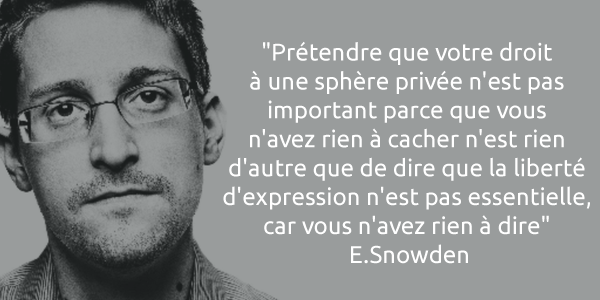
\includegraphics[scale=0.4]{./images/snowden.png}
\end{center}
\begin{itemize}
\item Snowden et ses révélations (NSA)
\item La loi Renseignement en France...
\end{itemize}
\end{frame}

\begin{frame}
\frametitle{L'espionnage 2/2}
\begin{itemize}
\item Notre voisin
\item Notre "ex"
\item Notre collègue de boulot...
\end{itemize}
\end{frame}

\begin{frame}
\frametitle{La différence entre la vie privée et la sécurité en une image}
\begin{center}
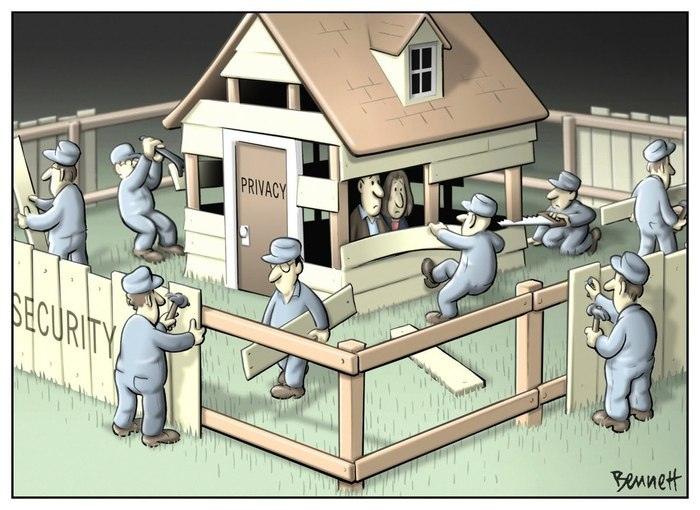
\includegraphics[scale=0.4]{./images/Security_Privacy.jpg}
\end{center}
\end{frame}

\begin{frame}
\Huge{\centerline{Faites-vous votre propre avis}}
\end{frame}


%========================================================================================
\begin{frame}
\Huge{\centerline{Comment se protéger ?}}
\Huge{\centerline{Un peu d'hygiène numérique}}
\end{frame}

%----------------------------------------------------------------------------------------
\begin{frame}
\frametitle{L'hygiène numérique?}
\begin{block}{}
\justifying{
L'hygiène est un ensemble de mesures destinées à prévenir les infections et l'apparition de maladies infectieuses.
\\
Ce guide d''hygiène numérique, ce sont des règles destinées à mieux utiliser son ordinateur, en sécurité, de façon simple.
}
\end{block}
\end{frame}

%----------------------------------------------------------------------------------------
\begin{frame}

\frametitle{Les mots de passe}
\begin{block}{Règles}
\begin{itemize}
\justifying{
\item Plus c'est long, plus c'est bon
\item Ne pas avoir le même mot de passe pour deux comptes en ligne.
}
\end{itemize}
\end{block}

\begin{block}{Mot de passe oublié?}
\justifying{
Pour tester la sécurité d'un site web, on clique sur le lien "mot de passe oublié".
\begin{itemize}
\item Si le mot de passe est renvoyé dans le mail, ce n'est pas bon. Le mot de passe est stocké en "clair".
\end{itemize}
}
\end{block}

\begin{block}{Trop de mot de passe à retenir?}
Il y a le logiciel Keepass. \url{http://www.keepass.info}
\end{block}

\end{frame}

%----------------------------------------------------------------------------------------
\begin{frame}
\frametitle{Navigateur}

Utilisez un navigateur respectueux de nos données personnelles : Firefox.

\begin{block}{Pourquoi Firefox?}
\justifying{
\begin{itemize}
\item La navigation privée permet de ne pas garder de traces sur l'ordinateur (mais ça ne suffit pas).
\item On peut ajouter des extensions anti-tracking et anti-pubs (Ghostery/Request Policy, Adblock...)
\end{itemize}
}
\end{block}
\justifying{}
\end{frame}

%----------------------------------------------------------------------------------------
\begin{frame}
\begin{center}
\Huge{Installer des extensions \\ pour Firefox }
\end{center}
\end{frame}

%----------------------------------------------------------------------------------------
\begin{frame}
\frametitle{AdBlock - block 1/2}
Page avec publicité :
\begin{center}
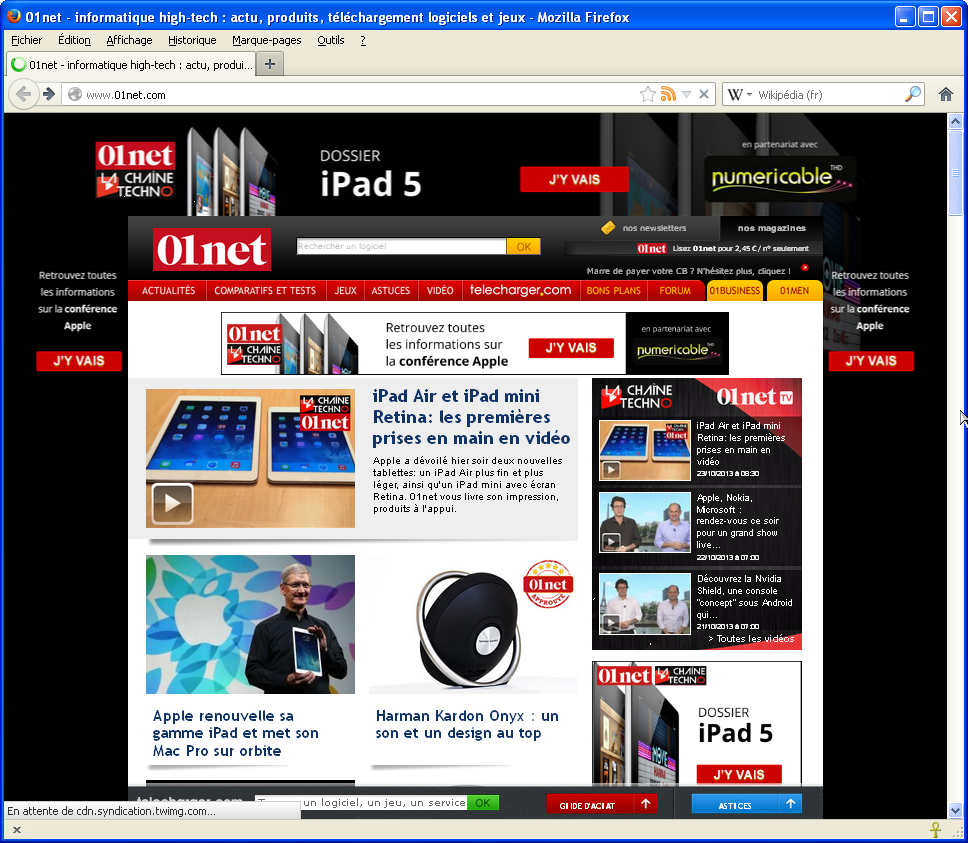
\includegraphics[scale=0.4] {./images/Adblock01.png}
\end{center}

\end{frame}

%----------------------------------------------------------------------------------------
\begin{frame}
\frametitle{AdBlock - Microblock 2/2}
Bloque les publicités. Allège les pages.

\begin{center}
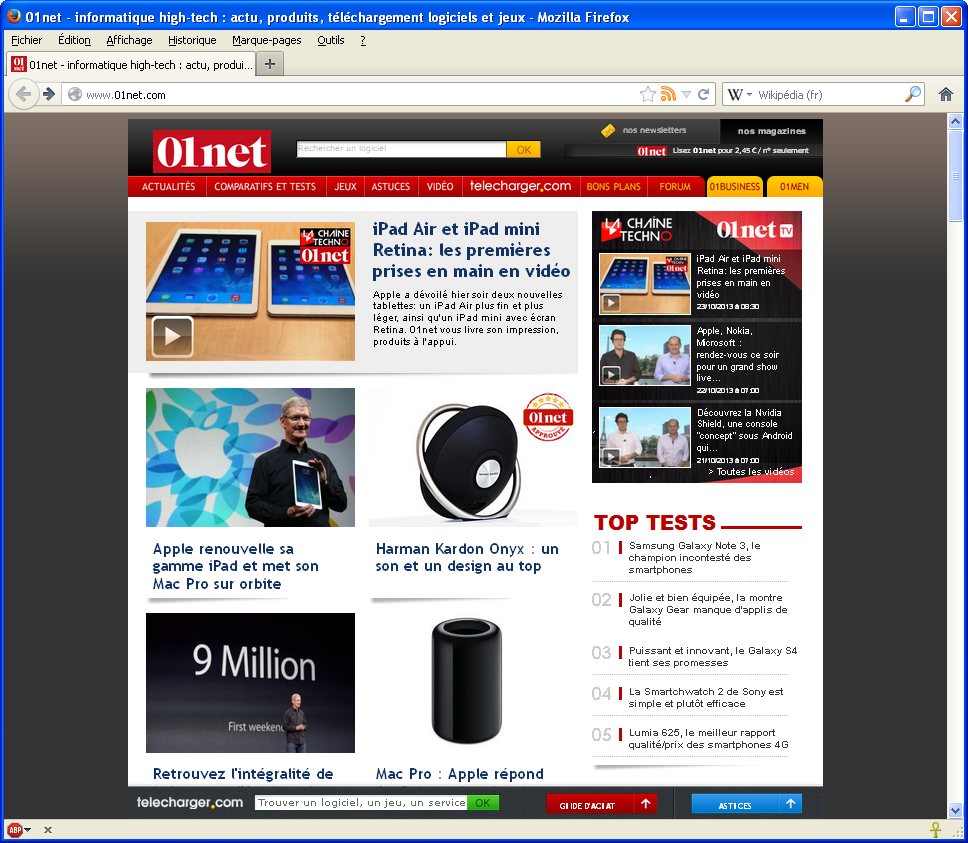
\includegraphics[scale=0.4] {./images/Adblock02.png}
\end{center}
\end{frame}

%----------------------------------------------------------------------------------------
\begin{frame}
\frametitle{Ghostery}

Bloque tous les trackers associés au site.
\begin{center}
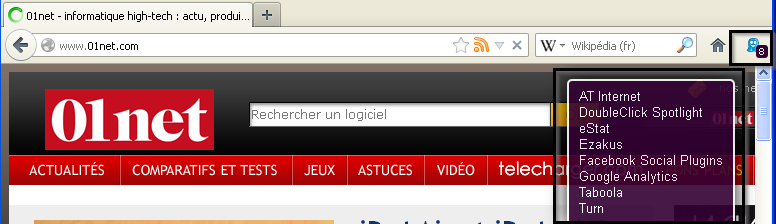
\includegraphics[scale=0.4] {./images/Ghostery_tracker.png}
\end{center}
\end{frame}

%----------------------------------------------------------------------------------------
\begin{frame}
\frametitle{HttpsEverywhere}

Avoir une connexion httpS dès que possibe
\begin{center}
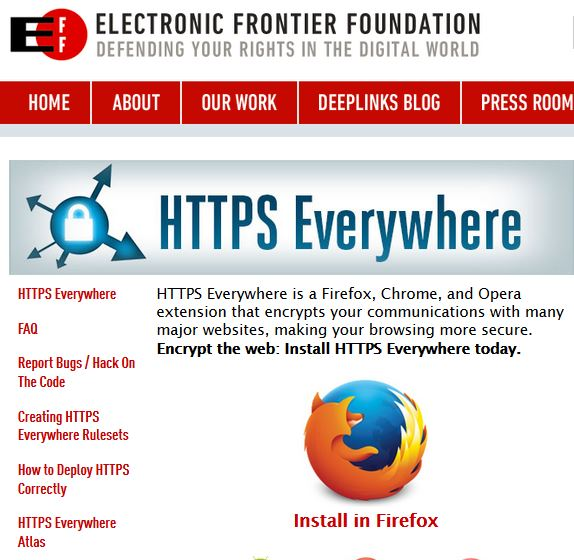
\includegraphics[scale=0.5] {./images/httpseverywhere.jpg}
\end{center}
\end{frame}
%----------------------------------------------------------------------------------------
\begin{frame}
\begin{center}
\Huge{Changer de moteur de recherche}
\end{center}
\end{frame}

%----------------------------------------------------------------------------------------
\begin{frame}
\frametitle{Utiliser des moteurs de recherche plus respectueux de la vie privée (DuckDuckGo...)}

\begin{block}{Les alternatives à Google}
\justifying{
\begin{itemize}
\item Duckduckgo \url{https://duckduckgo.com}
\item Qwant \url{https://www.qwant.com}
\item Framabee \url{https://framabee.org} ou TontonRoger \url{https://tontonroger.org/}
\end{itemize}
}
\end{block}
\end{frame}

%----------------------------------------------------------------------------------------
\begin{frame}
\begin{center}
\frametitle{Duckduckgo - Google tracks you. We don't.}

\url{https://duckduckgo.com}
\\
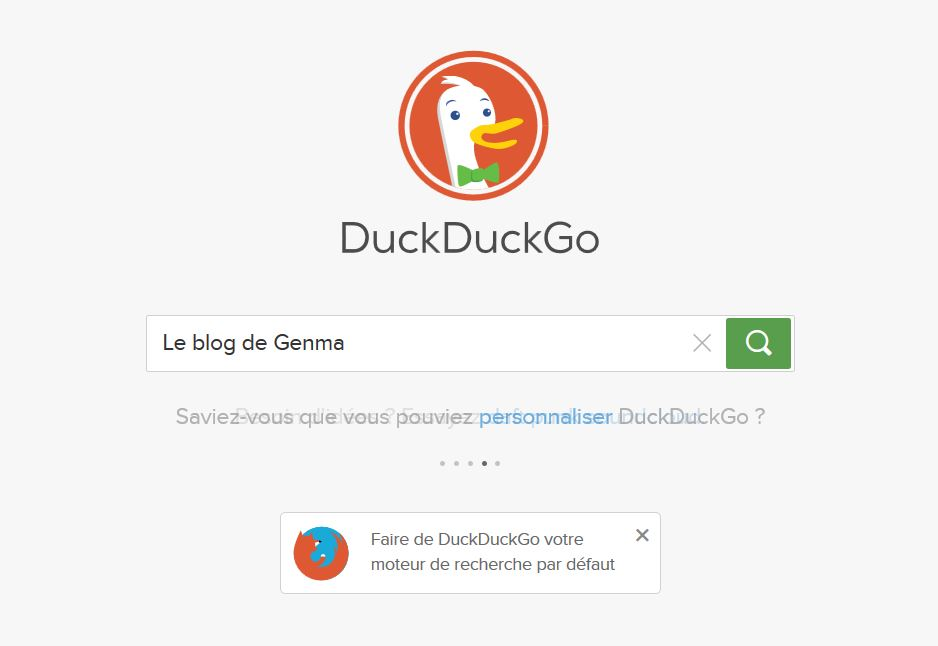
\includegraphics[scale=0.6] {./images/DuckDuckGo.jpg}
\end{center}
\end{frame}

\begin{frame}
\begin{center}
\frametitle{Framabee par Framasoft}

\url{https://framabee.org}
\\
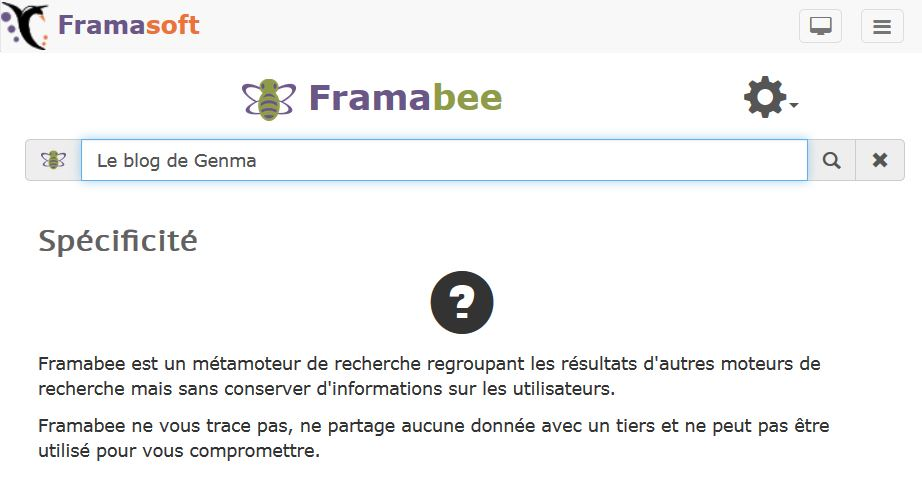
\includegraphics[scale=0.6] {./images/Framabee.jpg}
\end{center}
\end{frame}

\begin{frame}
\begin{center}
\frametitle{Qwant}

\url{https://qwant.com}
\\
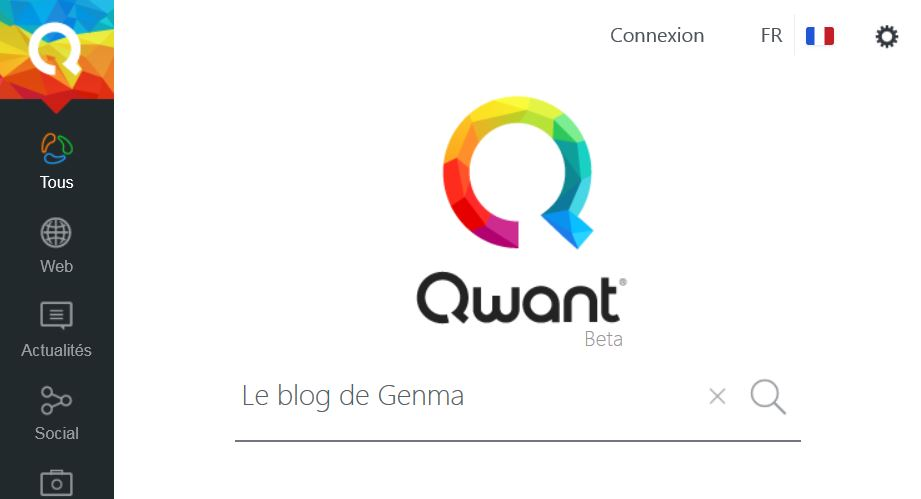
\includegraphics[scale=0.6] {./images/Qwant.jpg}
\end{center}
\end{frame}

%----------------------------------------------------------------------------------------
\begin{frame}
\begin{center}
\Huge{Utilisation d'Internet \\depuis un lieu public}
\end{center}
\end{frame}

 %----------------------------------------------------------------------------------------
\begin{frame}
\frametitle{Utilisation d'un PC d'un Cybercafé?}

\begin{block}{Pour le surf Internet}
\begin{itemize}
\justifying{
\item Éviter les sites sur lesquels on saisit des données personnelles : webmail, réseaux sociaux
\item Vérifier la version du navigateur
\item  Ne pas mémoriser vos informations confidentielles
\item  Penser à fermer votre session
\item  Effacer vos traces de navigation
}
\end{itemize}
\end{block}
\justifying{
Ne pas brancher de clef USB (virus), ne pas récupérer de documents.
\\
Idéalement ? Un navigateur en mode portable, depuis une clef USB
\\
Encore mieux : rebooter sur un live-usb/cd
}
\end{frame}
%----------------------------------------------------------------------------------------
\begin{frame}
\frametitle{Wi-Fi public?}
Ne pas avoir confiance. Utiliser sa propre machine.
\begin{block}{Attention à la sécurisation}
\begin{itemize}
\justifying{
\item Au minimum : connexion HTTPS
\item Mieux, passer par un VPN
}
\end{itemize}
\end{block}
\end{frame}

%----------------------------------------------------------------------------------------
\begin{frame}
\begin{center}
\Huge{Changer de Cloud}
\end{center}
\end{frame}
%----------------------------------------------------------------------------------------
\begin{frame}
\begin{center}
\frametitle{Framasoft et tous ses outils de Degogglisons}
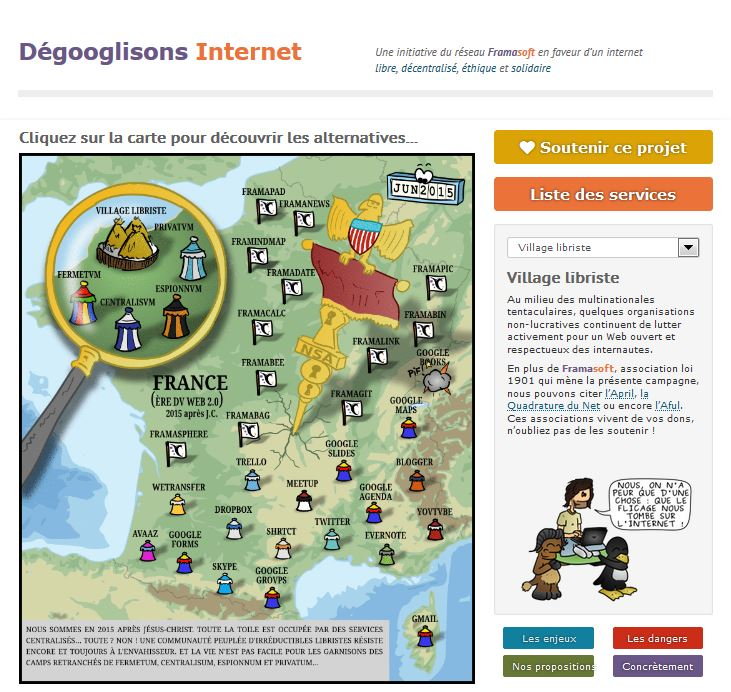
\includegraphics[scale=0.6] {./images/framasoft_degogglisons.jpg}
\end{center}
\end{frame}
%----------------------------------------------------------------------------------------
\begin{frame}
\begin{center}
\frametitle{Cozycloud}
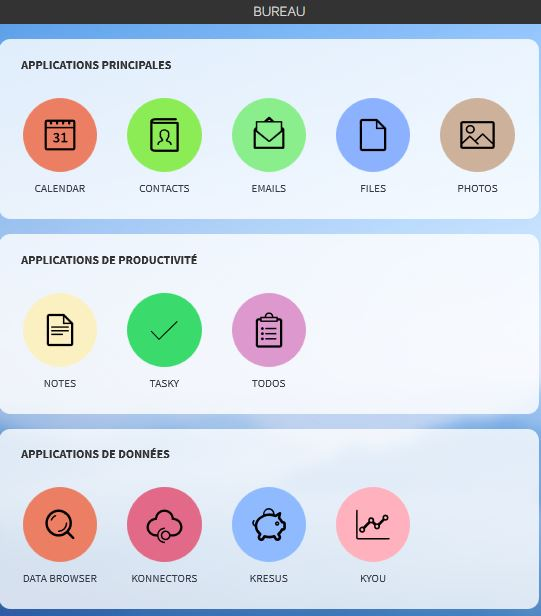
\includegraphics[scale=0.6] {./images/Cozycloud.jpg}
\end{center}
\end{frame}

%----------------------------------------------------------------------------------------
\begin{frame}
\begin{center}
\frametitle{Owncloud}
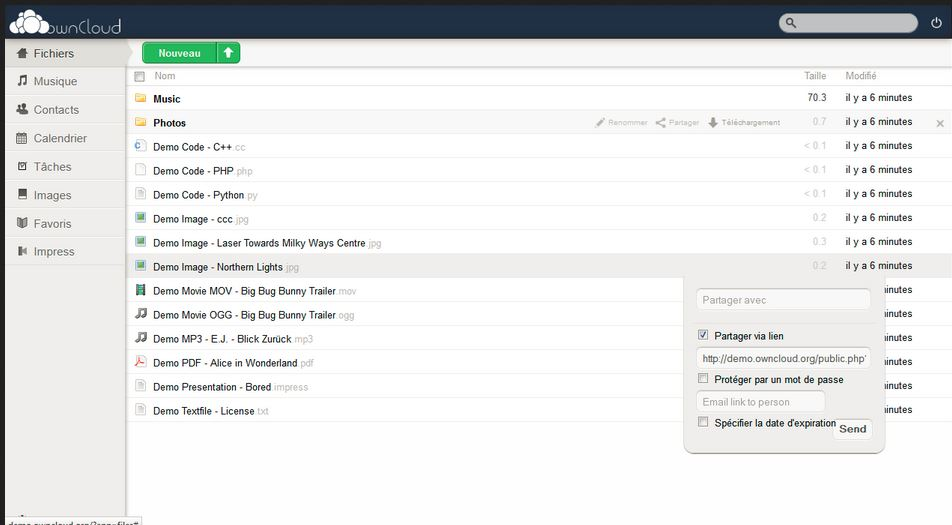
\includegraphics[scale=0.6] {./images/owncloud.jpg}
\end{center}
\end{frame}
%----------------------------------------------------------------------------------------
\begin{frame}
\begin{center}
\frametitle{La brique Internet}
\url{http://labriqueinter.net}
\\~\\
\includegraphics[scale=0.1] {./images/labriqueinternet.png}
\end{center}
\end{frame}

%----------------------------------------------------------------------------------------
\begin{frame}
\begin{center}
\Huge{Autres conseils }
\end{center}
\end{frame}

%----------------------------------------------------------------------------------------
\begin{frame}
\begin{center}
\Huge{Utiliser un pseudonyme }
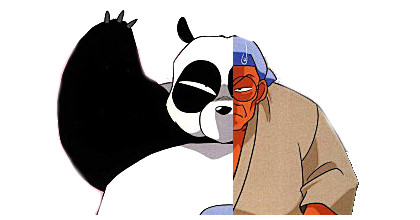
\includegraphics[scale=0.5] {./images/bannierepseudonymat.jpg}
\end{center}
\end{frame}

%----------------------------------------------------------------------------------------
\begin{frame}
\frametitle{Le pseudonymat}

\begin{block}{Défintions}
\begin{itemize}
\justifying{
\item Contraction des termes pseudonyme et anonymat, le terme de pseudonymat reflète assez bien la volonté contradictoire d’être un personnage public et de rester anonyme...
\item Un pseudonyme, c'est aussi une identité publique, qui est associée à un ensemble cohérent de comptes qui forment un tout : un blog, un compte Twitter, un compte Facebook...
}
\end{itemize}
Avoir un pseudonyme ne veut pas dire faire et dire n'importe quoi.
\\~\\Il en va de l'image que je renvoie, que je donne de moi et de ma crédibilité présente et à venir.
\end{block}
\end{frame}

%----------------------------------------------------------------------------------------
\begin{frame}
\frametitle{Les avantages du pseudonymat}

\begin{block}{Ce que permet le pseudonymat}
\justifying{Il permet de cloisonner sa vie numérique.}
\begin{itemize}
\justifying{
\item On a une une identité civile en ligne (nom prénom) avec le strict minimum.
\item Et une identité publique, un pseudonyme, qui permet d'avoir une activité plus fournie.
}
\end{itemize}
\end{block}
\justifying{
Ne pas oublier d'avoir une adresse mail qui n'est pas de la forme prénom.nom (sinon on perd l'intérêt du pseudonyme).
}
\end{frame}

%----------------------------------------------------------------------------------------
\begin{frame}
\frametitle{Plusieurs pseudonymes}

\justifying{
Quand on crée un compte sur un site, on peut envisager de saisir des informations nominatives spécifiques à ce site. On aura alors un pseudonyme par type de communauté fréquenté (jeu vidéo, informatique, de rencontres...).
\\~\\
S’il y a un problème (\emph{compte piraté}), on limitera le risque de diffusion des informations personnelles.
}
\end{frame}

%----------------------------------------------------------------------------------------
\begin{frame}
\frametitle{Pseudonymat et célébrité}

\justifying{Nombreuses sont les célébrités du monde de la télévision, cinéma, musique... Et Internet ?}
\begin{block}{Des pseudonymes internet \emph{connus}}
\begin{itemize}
\justifying{
\item Maitre Eolas, l'avocat
\item Zythom, l'expert judiciaire
\item Boulet, dessinateur
\item ...
}
\end{itemize}
\end{block}
\justifying{Et beaucoup d'autres, dans les communautés geek, hackers...}
\end{frame}

%----------------------------------------------------------------------------------------
\begin{frame}
\frametitle{Les limites du pseudonymat}

\begin{block}{Un pseudonymat c'est contraignant}

\justifying{On est très facilement tracés et reliés à sa véritable identité (via l'adresse IP).}
\begin{itemize}
\justifying{
\item Pour avoir un pseudonymat parfaitement cloisonné, il faut utiliser différentes techniques avancées...
}
\end{itemize}
\end{block}

\begin{block}{NE JAMAIS faire d'erreur}
\begin{itemize}
\justifying{
\item On ne dévoile pas son pseudonyme a des personnes qui connaissent notre identité civile.
\item On ne dévoile pas son visage en public....
}
\end{itemize}
\end{block}
\justifying{
Le pseudonymat est donc on ne peut plus relatif et tout dépend de ce que l'on souhaite comme pseudonymat.
}
\end{frame}

%----------------------------------------------------------------------------------------
\begin{frame}
\begin{center}
\Huge{Une solution simple reste d'être moins \emph{bavard}}
\end{center}
\end{frame}

%----------------------------------------------------------------------------------------
\begin{frame}
\begin{center}
\Huge{D'un peu plus complexe...\\ à très technique}
\end{center}
\end{frame}

\begin{frame}
\begin{center}

\includegraphics[scale=0.4] {./images/LogoCafeViePrivee.jpg}
\end{center}

\justifying{Chaque exemple cité après, c'est entre 1h à 3h d'ateliers...}
\end{frame}

%----------------------------------------------------------------------------------------
\begin{frame}
\frametitle{Chiffrer ses disque durs (TrueCrypt...)}
\begin{center}
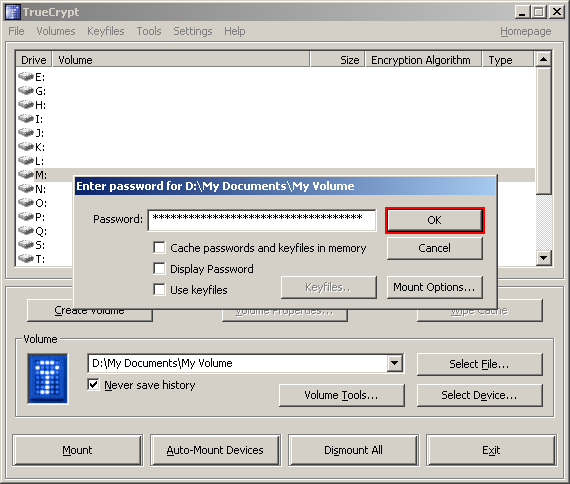
\includegraphics[scale=0.4] {./images/Truecrypt18.png}
\end{center}
\end{frame}

%----------------------------------------------------------------------------------------
\begin{frame}
\frametitle{Chiffrer ses disque durs (TrueCrypt...)}
\begin{center}
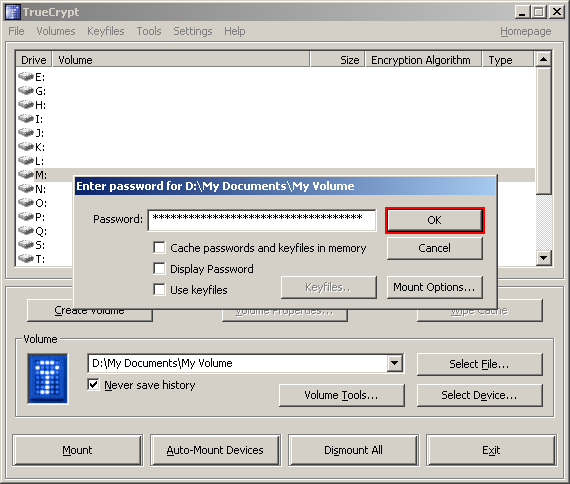
\includegraphics[scale=0.4] {./images/Truecrypt18.png}
\end{center}
\end{frame}

%----------------------------------------------------------------------------------------
\begin{frame}
\frametitle{Chiffrer ses mails  (GPG...)}
\begin{center}
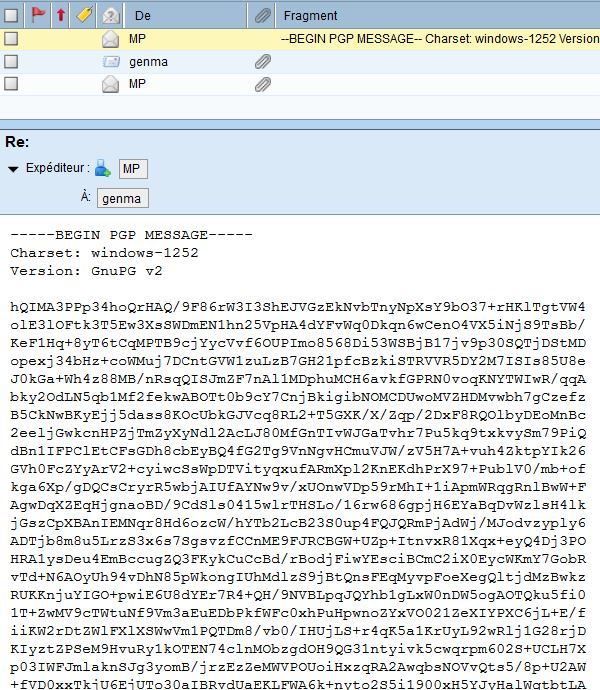
\includegraphics[scale=0.5] {./images/chiffrement_mail.jpg}
\end{center}
\end{frame}

%----------------------------------------------------------------------------------------
\begin{frame}
\frametitle{HttpS}
\begin{center}
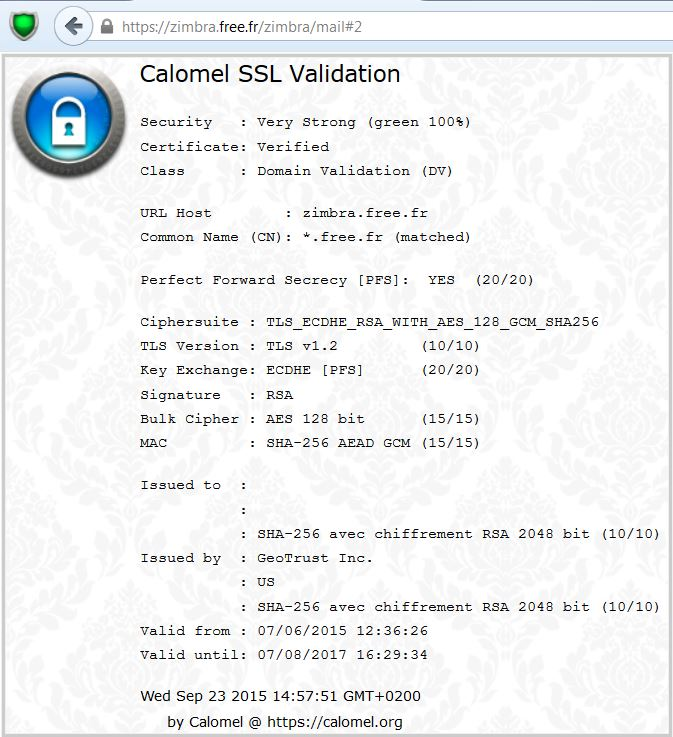
\includegraphics[scale=0.5] {./images/https.jpg}
\end{center}
\end{frame}

%----------------------------------------------------------------------------------------
\begin{frame}
\begin{center}
\Huge{Quelques mots sur Tor ? }
\\~\\ 
\includegraphics[scale=0.4]{./images/logo_tor.jpg}
\end{center}
\huge{Attention : la présentation \emph{complète} dure une bonne heure et demie...}
\end{frame}

%----------------------------------------------------------------------------------------
\begin{frame}
\frametitle{Comment fonctionne Tor ?}
\begin{center}
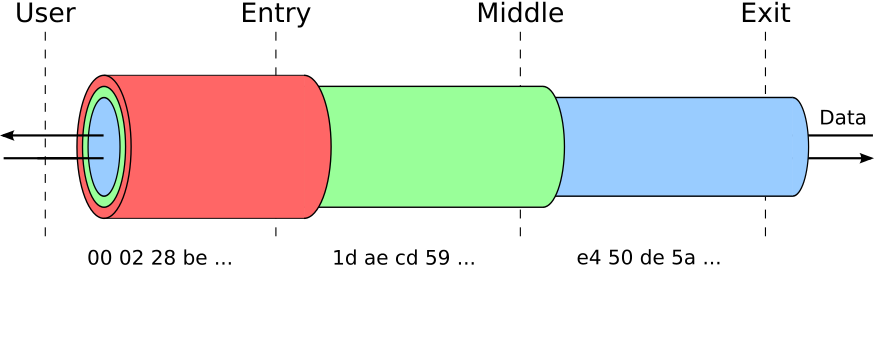
\includegraphics[keepaspectratio,width=\textwidth, height=.8\textheight]{images/tor-keys1}
\end{center}
\end{frame}

%----------------------------------------------------------------------------------------
\begin{frame}
\frametitle{A quoi sert TOR?}

\begin{block}{Ce que l'usage de Tor permet de faire}
\justifying{
\begin{itemize}
\justifying{
\item  d'échapper au fichage publicitaire,
\item  de publier des informations sous un pseudonyme,
\item  d'accéder à des informations en laissant moins de traces,
\item  de déjouer des dispositifs de filtrage (sur le réseau de son entreprise, de son Université, en Chine ou en France…),
\item  de communiquer en déjouant des dispositifs de surveillance,
\item  de tester son pare-feu,
\item  … et sûrement encore d'autres choses.
}
\end{itemize}
$\Rightarrow$ Tor dispose également d'un système de « services cachés » qui permet de fournir un service en cachant l'emplacement du serveur.
}
\end{block}
\end{frame}

%----------------------------------------------------------------------------------------
\begin{frame}
\frametitle{Télécharger le Tor Browser}
\justifying{
Toutes les versions (dans différentes langues, différents OS) sont disponibles sur le site du projet : 
\\ \url{https://www.torproject.org/}
\\ Rq : Il existe la possibilité de le recevoir par mail...
}
\begin{center}
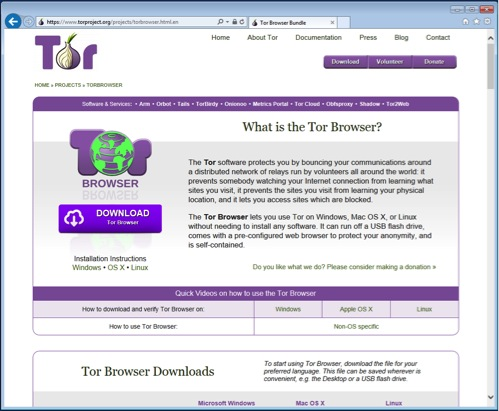
\includegraphics[scale=0.5]{./images/tor2.jpg}
\end{center}
\end{frame}

%----------------------------------------------------------------------------------------
\begin{frame}
\frametitle{Lancer le Tor Browser}
\begin{center}
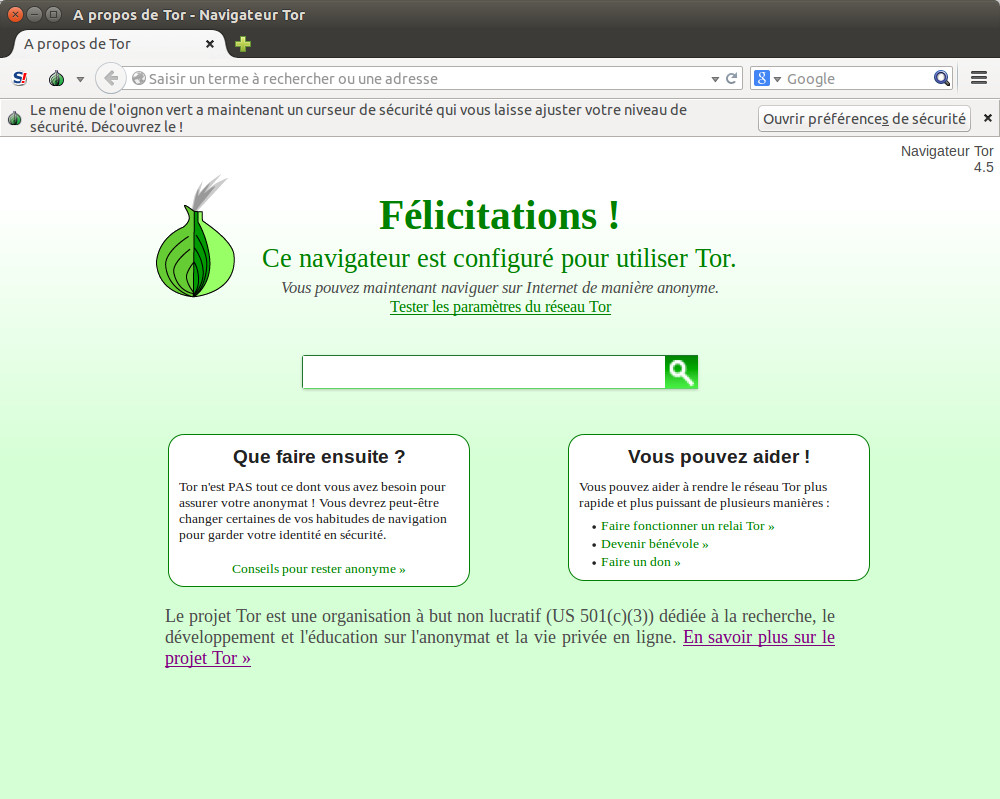
\includegraphics[scale=0.3]{./images/tor_browser03.jpg}
\end{center}
\end{frame}
%----------------------------------------------------------------------------------------

\begin{frame}
\frametitle{Utiliser Tor - Tails}
\justifying{
Tails (The Amnesic Incognito Live System) est un système d'exploitation complet basé sur Linux et Debian, en live.
}
\begin{center}
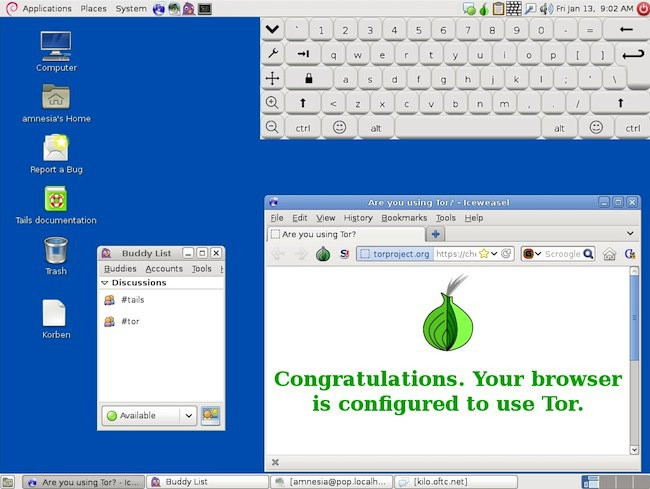
\includegraphics[scale=0.3]{./images/tails.jpg}
\\~\\
\url{https://tails.boom.org}
\end{center}
\end{frame}

%----------------------------------------------------------------------------------------
\begin{frame}
\Huge{\centerline{Merci de votre attention.}}
\Huge{\centerline{Place aux questions.}}
\end{frame}

%----------------------------------------------------------------------------------------
\begin{frame}
\frametitle{\includegraphics[scale=0.4]{./images/Genma.jpg} \ \ \  Me contacter?}
\Huge{\centerline{Le Blog de Genma}}
\Huge{\centerline{http://genma.free.fr}}
\Huge{\centerline{~}}
\Huge{\centerline{Twitter : @genma}}
\end{frame}

%============================================================================================
\begin{frame}
\Huge{\centerline{ANNEXES}}
\end{frame}

\begin{frame}
\Huge{\centerline{Framasoft et la dégooglisation}}
\end{frame}

\begin{frame}
\frametitle{Les fonctionnalités existantes  1/2}
\begin{itemize}
\justifying{
\item \textbf{Framindmap} basé sur Wisemapping pour vos mind mapping (organisation d'idées)
\item \textbf{Framadate} basé sur Doodle qui permet de convenir d'un rendez-vous / réunion
\item \textbf{Framapad} basé sur Etherpad Lite pour éditer des documents à plusieurs
\item \textbf{Framanews} basé sur TinyTinyRSS pour suivre vos flux RSS
\item \textbf{Framacalc} basé sur Ethercalc pour éditer à plusieurs vos tableaux
\item \textbf{Framavectoriel} basé sur SVG-Edit pour créer vos images vectorielles
\item \textbf{Framasphère} basé sur Diaspora pour remplacer Facebook
\item \textbf{Framabag} basé sur Wallabag pour remplacer Pocket
\item \textbf{Frama.link} basé sur LSTU pour faire du raccourcissement d'URL
}
\end{itemize}
\end{frame}

\begin{frame}
\frametitle{Les fonctionnalités existantes 2/2}
\begin{itemize}
\justifying{
\item \textbf{Framadrive} basé sur Owncloud pour faire de l'hébergement de fichiers (et remplacer Google Drive, Dropbox...etc)
\item \textbf{Framagit} basé sur Gitlab et destiné à remplacer des hébergeurs de code comme Github
\item \textbf{Framabookin} basé sur BicBucStriim et destiné à remplacer les Google Books and co
\item \textbf{Framabee} basé sur un Searx et qui permet de faire des recherches sur le web
\item \textbf{Framapic} basé sur Lut.im qui permet d'héberger ses images
\item \textbf{Framabin} basé sur Zerobin qui permet de partager des bouts de textes comme sur Pastebin
\item \textbf{Framaboard} basé sur Kanboard qui permet de faire de la gestion de projets
\item \textbf{Framagames} pour les joueurs qui aiment les petits jeux libres
\item \textbf{Framatube} basé sur Mediagoblin pour partager des vidéos en ligne
}
\end{itemize}
\end{frame}
%----------------------------------------------------------------------------------------
\begin{frame}
\frametitle{Les prochaines fonctionnalités 1/2}
\begin{itemize}
\justifying{
\item \textbf{Framapétition} basé sur un Drupal avec WebForm pour lancer des pétitions
\item \textbf{Framatalk} basé sur Jitsi Meet qui vous permettra de discuter avec vos pôtes
\item \textbf{Framadrop} qui sort ce vendredi, basé sur LUFI qui permet de faire de l'hébergement temporaire de fichiers comme WeTransfer
\item \textbf{Framasites} basé sur PluXML pour héberger votre site web
\item \textbf{Framagenda} basé sur Webcalendar pour faire de l'agenda partagé
\item \textbf{Framacarte} basé sur uMap pour remplacer les Google Maps and co
\item \textbf{Framaslides} basé sur Strut.io pour faire des diaporamas
\item \textbf{Framameet} basé sur WanaWana pour organiser des évéments
\item \textbf{Framaloomio} basé sur Loomio pour faire de la prise de décisions
}
\end{itemize}
\end{frame}

%----------------------------------------------------------------------------------------
\begin{frame}
\frametitle{Les prochaines fonctionnalités 2/2}
\begin{itemize}
\justifying{
\item \textbf{Framatweet} basé sur Twister afin de remplacer tout ce qui est microblogging (Twitter)
\item \textbf{Frama-???} basé sur Scrumblr pour organiser ses idées
\item \textbf{Frama-???} basé sur WebODF ou PDFy pour faire du partage de PDF et remplacer des services comme Scribd
\item \textbf{Framapoulpe} basé sur Pootle pour organiser de la traduction de logiciels
\item \textbf{Framanotes} basé sur Laverna pour faire de la prise de note comme sur Evernote
\item \textbf{Framamail} basé sur Caliopen pour héberger vos emails
\item \textbf{Framaforms} basé sur Drupal avec WebForm pour créer des questionnaires / formulaires en ligne
\item \textbf{Framalistes} basé sur Sympa pour faire de la liste de diffusion
\item \textbf{Frama-???} basé sur JsBin pour partager du code et le debugguer à plusieurs
}
\end{itemize}
\end{frame}
%----------------------------------------------------------------------------------------

\begin{frame}
\Huge{\centerline{La navigation en mode privée}}
\end{frame}

%----------------------------------------------------------------------------------------
\begin{frame}
\frametitle{La navigation en mode privée 1/2}

\justifying{
\begin{block}{Quelles données ne sont pas enregistrées durant la navigation privée ?}
\begin{itemize}
\item pages visitées ;
\item saisies dans les formulaires et la barre de recherche ;
\item mots de passe ; 
\item liste des téléchargements ; 
\item cookies ;
\item fichiers temporaires ou tampons.
\end{itemize}
\end{block}
}
\end{frame}

%----------------------------------------------------------------------------------------
\begin{frame}
\frametitle{La navigation en mode privée 2/2}
\begin{center}
\includegraphics[scale=0.5] {./images/Navigation_privee.jpg} 
\end{center}
\end{frame}


%----------------------------------------------------------------------------------------
\begin{frame}
\frametitle{Effacer ses métadonnées}

\begin{block}{Effacer de façon sécurisée}
\justifying{
\begin{itemize}
\item Pour le formatage : Shred
\item Pour les métadonnées : MAT
\end{itemize}
}
\end{block}
\justifying{}
\end{frame}

%------------------------------------------------
\begin{frame}
\frametitle{Le logiciel MAT}
\begin{block}{Le logiciel MAT}
\justifying{
MAT est une boîte à outil composé d'une interface graphique, d'une version en ligne de commande et d'une bibliothèque.
\\~\\
MAT crée automatiquement une copie des documents originaux dans une version nettoyée (laissant intacts les originaux). 
\\~\\
MAT est fourni par défaut dans le live-cd Tails. 
}
\end{block}
\end{frame}

%------------------------------------------------
\begin{frame}
\frametitle{Le logiciel MAT}
\begin{center}
\includegraphics[scale=0.3] {./images/Mat.png} 
\end{center}
\end{frame}


%------------------------------------------------
\begin{frame}
\frametitle{Comment vérifier rapidement la sécurité d'un site ?}
\begin{block}{La check-liste}
\begin{itemize}
\justifying{
\item Le site a-t-il une connexion en https ? (SSL).
\item Y-a-t-il intégration d'éléments extérieurs au site en lui-même ?
\item Le site utilise-t-il Google Analytics ?
\item Le site utilise-t-il Google Fonts ?
\item Le site utilise-t-il des régies publicitaires ?
\item Le site utilise-t-il Cloudflare ?
\item Le DNS est-il géré par Cloudflare ?
\item Le site présente-t-il une politique de confidentialité ?
\item Le site utilise-t-il les cookies ?
\item Le site utilise-t-il des scripts javascript ?
}
\end{itemize}
\end{block}
\end{frame}

%----------------------------------------------------------------------------------------
\begin{frame}
\frametitle{Certificate Patrol}
Permet de valider les certificats d'un site (lié à https).
\begin{center}
\includegraphics[scale=0.5] {./images/CertificatePatrol.png}
\end{center}
\end{frame}

%----------------------------------------------------------------------------------------
\begin{frame}
\frametitle{Certificate Patrol}
\begin{center}
\includegraphics[scale=0.5] {./images/Certificate_Patrol_certifcat_a_change.jpg}
\end{center}
\end{frame}

%----------------------------------------------------------------------------------------
\begin{frame}
\frametitle{Calomel SSL}
\begin{center}
\includegraphics[scale=0.5] {./images/Calomel.jpg}
\end{center}
\end{frame}

%----------------------------------------------------------------------------------------
\begin{frame}
\Huge{\centerline{L'authentification forte}}
\end{frame}

\begin{frame}
\frametitle{L'authentification forte}

\begin{block}{Différents termes, un même usage}
Double authentification, Connexion en deux étapes, 2-Step Verification
\end{block}

\begin{block}{Exemple avec Google} 
\justifying{
Google permet aux utilisateurs d'utiliser un processus de vérification en deux étapes.
\begin{itemize}
\item La première étape consiste à se connecter en utilisant le nom d'utilisateur et mot de passe. Il s'agit d'une application du facteur de connaissance.
\item Au moment de la connexion Google envoit par SMS un nouveau code unique. Ce nombre doit être entré pour compléter le processus de connexion. 
\end{itemize}
Il y a aussi une application à installer qui génère un nouveau code toutes les 30 secondes.
}
\end{block}
\end{frame}

%----------------------------------------------------------------------------------------
\begin{frame}
\frametitle{L'authentification forte}
\begin{block}{Autres services implémentant cette fonctionnalité}
\begin{itemize}
\item Web : Facebook, Twitter, Linkedin, Paypal
\item Banque : envoit d'un code par SMS
\end{itemize}
\end{block}
\end{frame}



%============================================================================================
\end{document}
